\documentclass{article}
\usepackage{graphicx}
\title{Analysis of Clustering Agent Implementation for Assignment 3}
\author{Jason Tellis}
\date{\today}
\begin{document}

\begin{figure}
  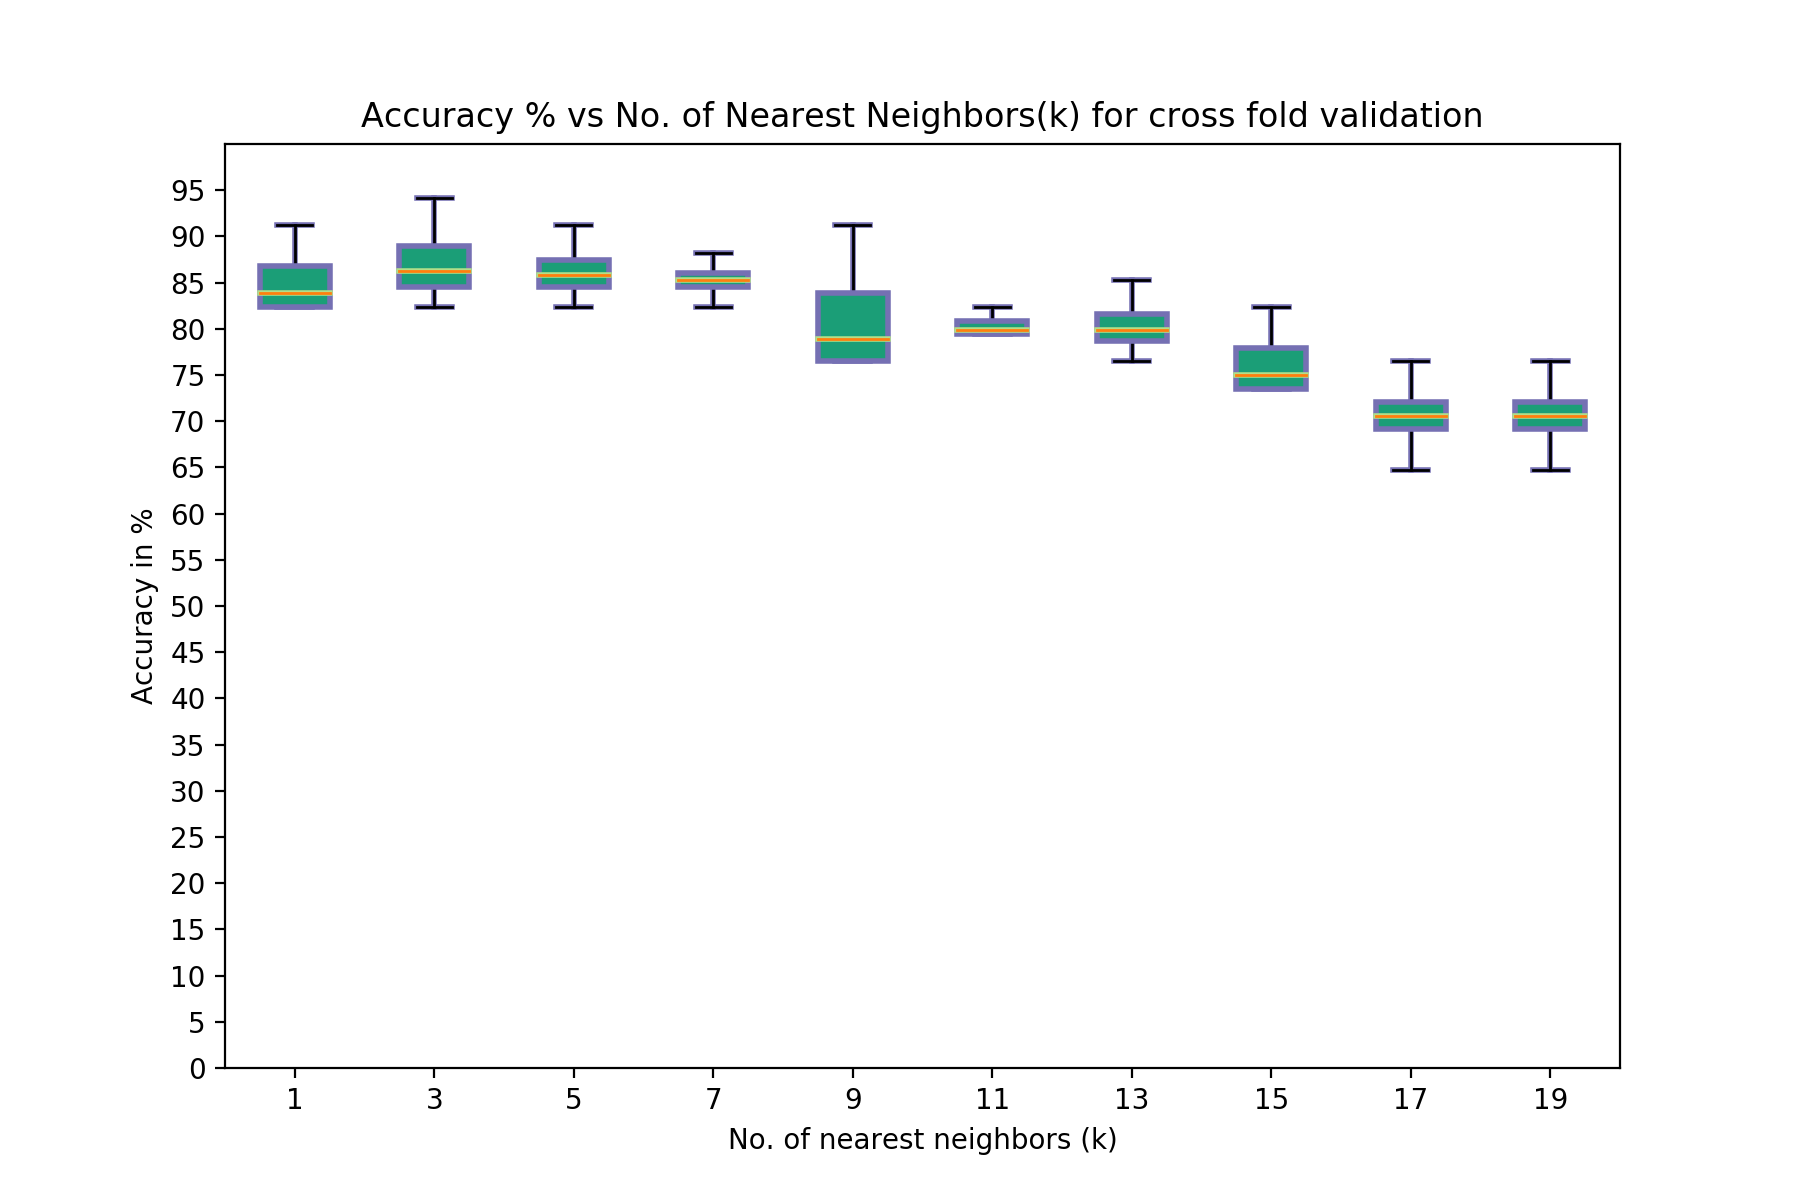
\includegraphics[width=\linewidth]{accuracy_plot_k=20.png}
  \caption{Box and Whiskers Plot of accuracy vs No. of Nearest Neighbors}
\end{figure}

\section{K-Means Clustering}
Two clusters are formed:
1 with with 23 headshot and 28 landscapes,
Other with 23 landscape ,28 headshot ,

While the cohesion or separation is not very high, both clusters do have opposing classes as majority members distinguishing one as dominated by headshots and other as dominated by landscapes


\section{Hierarchical Clustering for Headshots and Landscapes}
Two clusters are formed:
1 with just one image and other with the remaining images

This seems to be an issue with the dataset or the algorithm used as repeated trials produce similar clustering.
The performance of the clustering agent in this case is poorer than that of the K Means Agent

\section{Hierarchical Clustering for Flags}
Performance is identical to that of performance for Headshots and Landscapes.
Overall performance seems to be quite poor


\end{document}
